%\documentclass[dvipdfmx]{beamer}      % platex の場合
\documentclass{beamer}                 % lualatex の場合
\usepackage{mySld}

\begin{document}
\title{基礎コンピュータ工学\\第2章 情報の表現\\(パート4)}
\date{}

\begin{frame}
  \titlepage
  \centerline{\url{https://github.com/tctsigemura/TecTextBook}}
  \vfill
  \centerline{本スライドの入手:
    \raisebox{-7mm}{
\includegraphics[scale=0.3]{../Img/QRs2_4.png}}}
\end{frame}

%==============================================================================
%\begin{frame}
%  \frametitle{}
%\end{frame}

\section{情報の表現}
%==============================================================================
\begin{frame}
  \frametitle{2進数の和差の計算(復習)}

\emph{2進数の場合}は以下のようになる.
  \begin{itemize}
  \item 1より大きくなる時に\emph{桁上げ}が発生する.

    \texttt{
    \begin{tabular}{l l}
        & 010 \\
      + & 001 \\
      \cline{1-2}
        & 011
    \end{tabular}~~
    \begin{tabular}{l l}
        & 001 \\
      + & 001 \\
      \cline{1-2}
        & 010
    \end{tabular}~~
    \begin{tabular}{l l}
        & 010 \\
      + & 011 \\
      \cline{1-2}
        & 101
    \end{tabular}~~
    \begin{tabular}{l l}
        & 011 \\
      + & 001 \\
      \cline{1-2}
        & 100
    \end{tabular}~~
    \begin{tabular}{l l}
        & 011 \\
      + & 011 \\
      \cline{1-2}
        & 110
    \end{tabular}
    }

    \vfill
  \item \emph{桁借り}では2借りてくる.
    \texttt{
    \begin{tabular}{l l}
        & 011 \\
      - & 001 \\
      \cline{1-2}
        & 010
    \end{tabular}~~
    \begin{tabular}{l l}
        & 010 \\
      - & 001 \\
      \cline{1-2}
        & 001
    \end{tabular}~~
    \begin{tabular}{l l}
        & 101 \\
      - & 011 \\
      \cline{1-2}
        & 010
    \end{tabular}~~
    \begin{tabular}{l l}
        & 100 \\
      - & 001 \\
      \cline{1-2}
        & 011
    \end{tabular}~~
    \begin{tabular}{l l}
        & 110 \\
      - & 011 \\
      \cline{1-2}
        & 011
    \end{tabular}
    }

  \end{itemize}
\end{frame}

%==============================================================================
\begin{frame}[fragile]
  \frametitle{2進数の和差の計算(復習)}
  10進数の計算と2進数の計算をしなさい.
    \begin{minipage}{0.48\columnwidth}
      \begin{itembox}[l]{3+8}
        \texttt{
          \begin{tabular}{r r}
            \multicolumn{2}{c}{10進} \\
              &  3 \\
            + &  8 \\
            \cline{1-2}
              &
          \end{tabular}~~~
          \begin{tabular}{r r}
            \multicolumn{2}{c}{2進} \\
              & 0011 \\
            + & 1000 \\
            \cline{1-2}
              &
          \end{tabular}
        }
      \end{itembox}
    \end{minipage}
    \begin{minipage}{0.48\columnwidth}
      \begin{itembox}[l]{5+7}
        \texttt{
          \begin{tabular}{r r}
            \multicolumn{2}{c}{10進} \\
              &  5 \\
            + &  7 \\
            \cline{1-2}
              &
          \end{tabular}~~~
          \begin{tabular}{r r}
            \multicolumn{2}{c}{2進} \\
              & 0101 \\
            + & 0111 \\
            \cline{1-2}
              &
          \end{tabular}
        }
      \end{itembox}
    \end{minipage}\\
    \begin{minipage}{0.48\columnwidth}
      \begin{itembox}[l]{11-8}
        \texttt{
          \begin{tabular}{r r}
            \multicolumn{2}{c}{10進} \\
              & 11 \\
            - &  8 \\
            \cline{1-2}
              &
          \end{tabular}~~~
          \begin{tabular}{r r}
            \multicolumn{2}{c}{2進} \\
              & 1011 \\
            - & 1000 \\
            \cline{1-2}
              &
          \end{tabular}
        }
      \end{itembox}
    \end{minipage}
    \begin{minipage}{0.48\columnwidth}
      \begin{itembox}[l]{12-7}
        \texttt{
          \begin{tabular}{r r}
            \multicolumn{2}{c}{10進} \\
              & 12 \\
            - &  7 \\
            \cline{1-2}
              &
          \end{tabular}~~~
          \begin{tabular}{r r}
            \multicolumn{2}{c}{2進} \\
              & 1100 \\
            - & 0111 \\
            \cline{1-2}
              &
          \end{tabular}
        }
      \end{itembox}
    \end{minipage}
\end{frame}

%==============================================================================
\begin{frame}
  \frametitle{負の数を含む計算}
  \emph{2の補数表現の負数は符号無し2進数と同じ手順で計算できる!!}
  \vfill
  \begin{itemize}
  \item 最上位ビットからの桁上げは\emph{無視}する.

    \texttt{
    \begin{tabular}{c r r}
        & 0010 & (+2)\\
      + & 1111 & (-1)\\
      \cline{1-2}
        & 0001 & (+1)
    \end{tabular}~~
    \begin{tabular}{c r r}
        & 1011 & (-5) \\
      + & 0101 & (+5) \\
      \cline{1-2}
        & 0000 & (+0)
    \end{tabular}~~
    \begin{tabular}{c r r}
        & 1101 & (-3) \\
      + & 1101 & (-3) \\
      \cline{1-2}
        & 1010 & (-6)
    \end{tabular}
    }
    \vfill
  \item 仕組み
    \begin{itemize}
    \item \emph{正の数と負の数の和}(-b を2の補数$(2^n - b)$と表現する)\\
      正の値aと負の値-bの和を計算し$2^n$(最上位の桁上げ)を無視する\\
      \centerline{$a + (-b) = a + (2^n - b) = 2^n + a - b = a - b$}
    \item \emph{負の数と負の数の和}(-a,-b を2の補数で表現する)\\
      $2^n$(最上位からの桁上げ)を一つ無視すると\\
      $(-a) + (-b) = (2^n - a) + (2^n - b) = 2^n - (a + b)$
    \end{itemize}
  \end{itemize}
\end{frame}

%==============================================================================
\begin{frame}
  \frametitle{負の数を含む計算}
  \emph{2の補数表現の負数は符号無し2進数と同じ手順で計算できる!!}
  \vfill
  \begin{itemize}
  \item 最上位ビットの桁借りは\emph{制限なし}とする.

    \texttt{
    \begin{tabular}{c r r}
        & 0010 & (+2)\\
      - & 1111 & (-1)\\
      \cline{1-2}
        & 0011 & (+3)
    \end{tabular}~~
    \begin{tabular}{c r r}
        & 0000 & (+0) \\
      - & 0101 & (+5) \\
      \cline{1-2}
        & 1011 & (-5)
    \end{tabular}~~
    \begin{tabular}{c r r}
        & 1101 & (-3) \\
      - & 1010 & (-6) \\
      \cline{1-2}
        & 0011 & (+3)
    \end{tabular}
    }
    \vfill
  \item 仕組み
    \begin{itemize}
    \item \emph{正の数と負の数の差}(-b を2の補数$(2^n - b)$と表現する)\\
      正の値aと負の値-bの差を計算し$-2^n$(最上位の桁借り)を許す\\
      \centerline{$a - (-b) = a - (2^n - b) = -2^n + a + b = a + b$}
    \item \emph{負の数と負の数の差}(-a,-b を2の補数で表現する)\\
      $2^n$(最上位からの桁上げ)を一つ無視すると\\
      $(-a) - (-b) = (2^n - a) - (2^n - b) = (-a) + b$
    \end{itemize}
  \end{itemize}
\end{frame}

%==============================================================================
\begin{frame}
  \frametitle{負数を含む計算(問題1/2)}
  \emph{問題11:}次の計算を2進数と10進数でしなさい.\\
  (ただし,2進数は2の補数表現形式になっている)

  {\small\begin{center}
    \begin{tabular}{ l c r  c c r }
      1) &   & $0011~0010_2$ &    &   & $\fbox{   }_{10}$ \\
         & + & $0011~0010_2$ & → & + & $\fbox{   }_{10}$ \\
      \cline{2-3} \cline{5-6}
         &   & $\fbox{    }_2$ & ~ &  & $\fbox{   }_{10}$
    \end{tabular}
  \end{center}}

  {\small\begin{center}
    \begin{tabular}{ l c r  c c r }
      2) &   & $1111~1111_2$ &    &   & $\fbox{   }_{10}$ \\
         & + & $1111~1111_2$ & → & + & $\fbox{   }_{10}$ \\
      \cline{2-3} \cline{5-6}
         &   & $\fbox{    }_2$ & ~ &  & $\fbox{   }_{10}$
    \end{tabular}
  \end{center}}
\end{frame}

%==============================================================================
\begin{frame}
  \frametitle{負数を含む計算(問題2/2)}

  {\small\begin{center}
    \begin{tabular}{ l c r  c c r }
      3) &   & $0110~0100_2$ &    &   & $\fbox{   }_{10}$ \\
         & + & $1001~1100_2$ & → & + & $\fbox{   }_{10}$ \\
      \cline{2-3} \cline{5-6}
         &   & $\fbox{    }_2$ & ~ &  & $\fbox{   }_{10}$
    \end{tabular}
  \end{center}}

  {\small\begin{center}
    \begin{tabular}{ l c r  c c r }
      4) &   & $1111~0000_2$ &    &   & $\fbox{   }_{10}$ \\
         & + & $1110~1111_2$ & → & + & $\fbox{   }_{10}$ \\
      \cline{2-3} \cline{5-6}
         &   & $\fbox{    }_2$ & ~ &  & $\fbox{   }_{10}$
    \end{tabular}
  \end{center}}

  {\small\begin{center}
    \begin{tabular}{ l c r  c c r }
      5) &     & $0001~0000_2$ &    &   & $\fbox{   }_{10}$ \\
         & $-$ & $1110~1111_2$ & → & $-$ & $\fbox{   }_{10}$ \\
      \cline{2-3} \cline{5-6}
         &     & $\fbox{    }_2$ & ~ &  & $\fbox{   }_{10}$
    \end{tabular}
  \end{center}}
\end{frame}

%==============================================================================
\begin{frame}
  \frametitle{2進数による小数の表現}
  \emph{固定小数点方式}(小数点の位置を\emph{約束}する.)
  \vfill
  \begin{quote}
    \begin{minipage}{0.4\columnwidth}
      $00.00_2 = 0.0_{10}$  \\
      $00.01_2 = 0.25_{10}$  \\
      $00.10_2 = 0.5_{10}$  \\
      $00.11_2 = 0.75_{10}$  \\
      $01.00_2 = 1.0_{10}$  \\
      $01.01_2 = 1.25_{10}$  \\
      $01.10_2 = 1.5_{10}$  \\
      $01.11_2 = 1.75_{10}$  \\
      $10.00_2 = 2.0_{10}$  \\
      ...\\
      $11.11_2 = 3.75_{10}$
    \end{minipage}
    \begin{minipage}{0.5\columnwidth}
      \emph{桁の重み}
      \begin{itemize}
      \item 小数点から左に進むと2倍
        $001.0000_2 = 1.0_{10}$ \\
        $010.0000_2 = 2.0_{10}$ \\
        $100.0000_2 = 4.0_{10}$ \\
        \vspace{1ex}
      \item 小数点から右に進むと1/2倍\\
        $000.1000_2 = 0.5_{10}$ \\
        $000.0100_2 = 0.25_{10}$ \\
        $000.0010_2 = 0.125_{10}$ \\
        $000.0001_2 = 0.0625_{10}$
      \end{itemize}
    \end{minipage}
  \end{quote}
\end{frame}

%==============================================================================
\begin{frame}
  \frametitle{固定小数点方式2進数 →  10進数}
  桁の重みを合計する.
  \begin{align}
    10.01_2 &= 1 \times 2 + 0 \times 1 + 0 \times 1/2 + 1 \times 1/4 \notag\\
            &= 2 + 0 + 0 + 1/4 \notag\\
            &= 2 + 0.25 \notag\\
            &= 2.25 \notag
  \end{align}
  \vfill
  \emph{問題12:}2進数を10進数に変換しなさい.
  \begin{enumerate}
  \item[1)] $0101.1010_2$
  \vfill
  \item[2)] $0011.0011_2$
  \vfill
  \item[3)] $0100.0101_2$
  \vfill
  \item[4)] $1010.1111_2$
  \end{enumerate}
\end{frame}

%==============================================================================
\begin{frame}
  \frametitle{10進数 →  固定小数点方式2進数}
  \centerline{\parbox{0.8\columnwidth}{\small
      \begin{center}
\begin{tabular}{ r l  l r}
\multicolumn{1}{c}{2進数} &  ~~~$\times 2$は~~~ & \multicolumn{2}{c}{10進数}\\
$0.101_2$ &        左シフ       &           & $0.625$ \\
\multicolumn{1}{c}{$\swarrow$} &   トと同じ     & $\times$  &     $2$ \\
\cline{3-4}
$1.010_2$      &                &           & $\underline{1}.250$ \\
&&&\\
\multicolumn{1}{c}{2進数} &  ~~~$\times 2$は~~~ & \multicolumn{2}{c}{10進数}\\
$0.010_2$ &        左シフ       &           & $0.250$ \\
\multicolumn{1}{c}{$\swarrow$} &   トと同じ     & $\times$  &     $2$ \\
\cline{3-4}
$0.100_2$      &                &           & $\underline{0}.500$ \\
&&&\\
\multicolumn{1}{c}{2進数} &  ~~~$\times 2$は~~~ & \multicolumn{2}{c}{10進数}\\
$0.100_2$ &        左シフ       &           & $0.500$ \\
\multicolumn{1}{c}{$\swarrow$} &   トと同じ     & $\times$  &     $2$ \\
\cline{3-4}
$1.000_2$      &                &           & $\underline{1}.000$ \\
\end{tabular}
      \end{center}
      10進数で計算したとき,小数点を横切って整数部に出てきた数を
      小数点の右に順番に並べると $0.\underline{101}_2$ になる.}}
\end{frame}

%==============================================================================
\begin{frame}
  \frametitle{固定小数点方式2進数 →  10進数}
  \emph{問題13:}10進数を2進数に変換しなさい.\\
       但し2進数は,小数点以下4桁,全体で6桁とする.
       \vfill
  \begin{enumerate}
  \item[1)] $0.75_{10}$
  \vfill
  \item[2)] $0.5625_{10}$
  \vfill
  \item[3)] $2.5_{10}$
  \vfill
  \item[4)] $1.1875_{10}$
  \end{enumerate}
\end{frame}

%==============================================================================
\begin{frame}
  \frametitle{文字の表現}
  \emph{ASCIIコード(American Standard Code for Information Interchange)}\\
  1963年にアメリカ規格協会(ANSI)が定めた情報交換用の文字コード.
%  英字,数字,記号等が含まれる.
%  今でもASCIIコードが基本になっている.
  
  \centerline{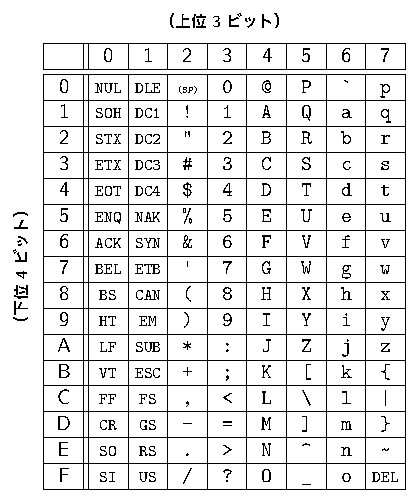
\includegraphics[scale=0.80]{../Tikz/ascii.pdf}}

\end{frame}

%==============================================================================
\begin{frame}
  \frametitle{文字の表現}
  \emph{JIS(Japan Industrial Standard:日本工業規格)8ビットコード}\\
  JIS 8ビットコードは,ASCIIコードに半角カタカナを追加したもの.
  記号,数字,英字の部分は,\.ほ\.ぼ,同じ並びになっている.

  \centerline{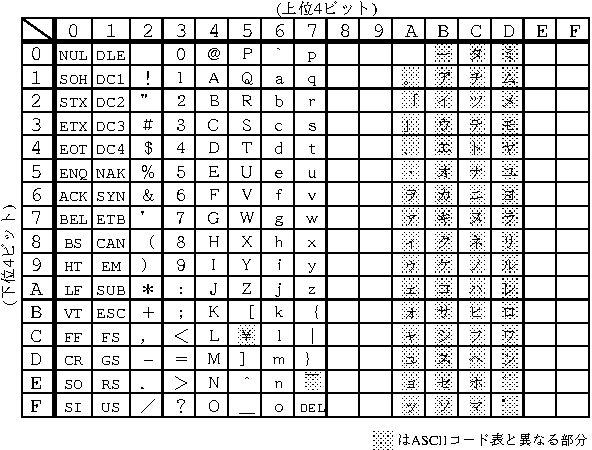
\includegraphics[scale=0.85]{../chap2/jisx0201.pdf}}

\end{frame}

%==============================================================================
\begin{frame}
  \frametitle{補助単位}
  1,000m を 1km,1,000g を 1kg, 0.001 l を 1ml, 0.001m を 1mm\\
  ここで,k や m は\emph{補助単位}と呼ばれる.\\

  \begin{center}
    {\small\begin{tabular}{r l l | r l l}\hline\hline
      \multicolumn{3}{c|}{一般的に} &
      \multicolumn{3}{c}{記憶容量} \\
      \hline
      \multicolumn{1}{c}{値} &
      \multicolumn{1}{c}{記号} &
      \multicolumn{1}{c|}{読み方} &
      \multicolumn{1}{c}{値} &
      \multicolumn{1}{c}{記号} &
      \multicolumn{1}{c}{読み方} \\
      \hline
      $10^3$   & $k$ & キロ   & $2^{10}$ & $Ki$ & キビ \\
      $10^6$   & $M$ & メガ   & $2^{20}$ & $Mi$ & メビ \\
      $10^9$   & $G$ & ギガ   & $2^{30}$ & $Gi$ & ギビ \\
      $10^{12}$& $T$ & テラ   & $2^{40}$ & $Ti$ & テビ \\
    \end{tabular}}
  \end{center}

  \begin{itemize}
  \item 通常は$10^3$毎に補助単位がある.
  \item コンピュータの記憶容量では$2^{10}$毎に補助単位がある.\\
    $2^{10} = 1,024 = 1Ki$ \\
    $10^3   = 1,000 = 1k$
  \end{itemize}
\end{frame}

\end{document}
